%%%%%%%%%%%%%%%%%%%%%%%%%%%%%%%%%%%%%%%%
% Jacobs Landscape Poster
% LaTeX Template
% Version 1.1 (14/06/14)
%
% Created by:
% Computational Physics and Biophysics Group, Jacobs University
% https://teamwork.jacobs-university.de:8443/confluence/display/CoPandBiG/LaTeX+Poster
% 
% Further modified by:
% Nathaniel Johnston (nathaniel@njohnston.ca)
%
% This template has been downloaded from:
% http://www.LaTeXTemplates.com
%
% License:
% CC BY-NC-SA 3.0 (http://creativecommons.org/licenses/by-nc-sa/3.0/)
%
%%%%%%%%%%%%%%%%%%%%%%%%%%%%%%%%%%%%%%%%%

%----------------------------------------------------------------------------------------
%	PACKAGES AND OTHER DOCUMENT CONFIGURATIONS
%----------------------------------------------------------------------------------------

\documentclass[final]{beamer}

\usepackage[scale=0.9]{beamerposter} % Use the beamerposter package for laying out the poster
\usepackage{listings}
\usetheme{confposter} % Use the confposter theme supplied with this template

\setbeamercolor{block title}{fg=ngreen,bg=white} % Colors of the block titles
\setbeamercolor{block body}{fg=black,bg=white} % Colors of the body of blocks
\setbeamercolor{block alerted title}{fg=white,bg=dblue!70} % Colors of the highlighted block titles
\setbeamercolor{block alerted body}{fg=black,bg=dblue!10} % Colors of the body of highlighted blocks
% Many more colors are available for use in beamerthemeconfposter.sty

%-----------------------------------------------------------
% Define the column widths and overall poster size
% To set effective sepwid, onecolwid and twocolwid values, first choose how many columns you want and how much separation you want between columns
% In this template, the separation width chosen is 0.024 of the paper width and a 4-column layout
% onecolwid should therefore be (1-(# of columns+1)*sepwid)/# of columns e.g. (1-(4+1)*0.024)/4 = 0.22
% Set twocolwid to be (2*onecolwid)+sepwid = 0.464
% Set threecolwid to be (3*onecolwid)+2*sepwid = 0.708

\newlength{\sepwid}
\newlength{\onecolwid}
\newlength{\twocolwid}
\newlength{\threecolwid}
\setlength{\paperwidth}{48in} % A0 width: 46.8in
\setlength{\paperheight}{36in} % A0 height: 33.1in
\setlength{\sepwid}{0.024\paperwidth} % Separation width (white space) between columns
\setlength{\onecolwid}{0.22\paperwidth} % Width of one column
\setlength{\twocolwid}{0.464\paperwidth} % Width of two columns
\setlength{\threecolwid}{0.708\paperwidth} % Width of three columns
\setlength{\topmargin}{-0.5in} % Reduce the top margin size
%-----------------------------------------------------------

\usepackage{graphicx}  % Required for including images

\usepackage{booktabs} % Top and bottom rules for tables
\usepackage{DejaVuSans}

%----------------------------------------------------------------------------------------
% TITLE SECTION
%----------------------------------------------------------------------------------------

\title{
Track-Centered Moving Grids for Tropical Cyclone Forecast Assessment
in the Model Evaluation Tools (MET) Verification Package} % Poster title

\author{David Fillmore} % Author(s)

\institute{National Center for Atmospheric Research,
Research Applications Lab} % Institution(s)

%----------------------------------------------------------------------------------------

\begin{document}

\addtobeamertemplate{block end}{}{\vspace*{2ex}} % White space under blocks
\addtobeamertemplate{block alerted end}{}{\vspace*{2ex}} % White space under highlighted (alert) blocks

\setlength{\belowcaptionskip}{2ex} % White space under figures
\setlength\belowdisplayshortskip{2ex} % White space under equations

\begin{frame}[containsverbatim] % The whole poster is enclosed in one beamer frame

\begin{columns}[t] % The whole poster consists of three major columns, the second of which is split into two columns twice - the [t] option aligns each column's content to the top

\begin{column}{\sepwid}\end{column} % Empty spacer column

\begin{column}{\onecolwid} % The first column

%----------------------------------------------------------------------------------------
%----------------------------------------------------------------------------------------

% \begin{alertblock}{Overview}
% \begin{itemize}
% \item
% \end{itemize}
% \end{alertblock}

%----------------------------------------------------------------------------------------
%----------------------------------------------------------------------------------------

\begin{figure}
\includegraphics[width=1.0\linewidth]{../plots/matthew_tmo_2016278_lrg.jpg}
% \caption{NASA Terra MODIS image of Hurricane Matthew on October 4, 2016.}
{\small NASA Terra MODIS image of Hurricane Matthew on October 4, 2016.}
\end{figure}

\begin{block}{Introduction}
Tropical cyclones, especially fully developed hurricanes,
exhibit quasi-stationary features with respect to the position of the storm center.
Such features include the eye-wall cloud, precipitation bands, and wind speed maxima.
Forecast model analysis and verification can thus benefit from statistics
aggregated on a moving range-azimuth grid centered on points along the storm track.
In this poster we will describe a new TC moving grid analysis tool
developed within the Developmental Testbed Center (DTC)
Model Evaluation Tools (MET) software suite.
MET is highly configurable and provides a variety of verification techniques
including standard verification scores comparing gridded model data
to gridded and point observations or re-analyses.
MET was chosen as the core of the National Oceanic and Atmospheric Administration (NOAA)
Unified Forecast System (UFS).
The larger system, METplus, includes the core MET tools,
python wrappers for automation over verification tasks,
a results database (METdb),
aggregation tools (METcalcpy),
and visualization tools (METplotpy, METviewer, METexpress).
\newline

This MET-TC tool supports several re-gridding methods,
storm track selection, and data aggregation or stratification based
on user specified criteria such as forecast initialization time.
Derived fields such as azimuthal means and the tangential
and radial wind components are computed.
The moving grid may also be rescaled along the track.
For example, the radial grid spacing may be set
as a factor of the radius of maximum winds.
\newline

As a case study we will present a 12-day (Sep. 28 – Oct. 9, 2016) analysis
of the Finite-Volume Cubed-Sphere 3 Global Forecast System (FV3GFS) forecasts
for Hurricane Matthew,
which intensified to a category 5 hurricane in the Caribbean Sea
and tracked along the southeast coast of the US,
where it continued to produce heavy rainfall and widespread flooding.
This dataset was created as a baseline case
for the Model Evaluation for Research Innovation Transition (MERIT) project,
with storm tracks generated from the Geophysical Fluid Dynamics Laboratory (GFDL)
vortex tracker.
The METplus modules, METcalcpy and METplotpy,
are used to examine the evolution of various surface
and pressure level quantities such as sea-level pressure,
precipitation, and surface and upper air wind fields.
Radial-vertical cross sections of azimuthally averaged quantities are also computed;
in particular, example statistics
and visualizations are generated for tangential winds,
radial and vertical mass and water vapor fluxes,
and equivalent potential temperature.

\end{block}

%----------------------------------------------------------------------------------------

\end{column} % End of the first column

\begin{column}{\sepwid}\end{column} % Empty spacer column

\begin{column}{\twocolwid} % Begin a column which is two columns wide (column 2)

\begin{columns}[t,totalwidth=\twocolwid] % Split up the two columns wide column

\begin{column}{\onecolwid}\vspace{-.6in} % The first column within column 2 (column 2.1)

%----------------------------------------------------------------------------------------

\end{column} % End of column 2.1

\begin{column}{\onecolwid}\vspace{-.6in} % The second column within column 2 (column 2.2)

%----------------------------------------------------------------------------------------

\end{column} % End of column 2.2

\end{columns} % End of the split of column 2 - any content after this will now take up 2 columns width

%----------------------------------------------------------------------------------------
% MET TC Tools
%----------------------------------------------------------------------------------------

\begin{alertblock}{MET TC Tools}
\begin{itemize}
\item {\bf TC Pairs} - Match TC forecast with reference TC data
(e.g. best track)
\item {\bf TC Stat} - Filter and create summary statistics
for TC Pairs output
\item {\bf TC Dland} - Compute gridded distance to land,
for use in TC Pairs and TC Stat filters
\item {\it New to MET 9.0}
{\bf TC Gen}, {\bf TC RMW}, {\bf RMW Analysis}
\end{itemize}
\end{alertblock}

%----------------------------------------------------------------------------------------

\begin{columns}[t,totalwidth=\twocolwid] % Split up the two columns wide column again

\begin{column}{\onecolwid} % The first column within column 2 (column 2.1)

%----------------------------------------------------------------------------------------
% TC RMW
%----------------------------------------------------------------------------------------

\begin{block}{TC RMW}

\begin{itemize}
\item Process model output with Automated Tropical Cyclone Forecast
(ATCF) track files, Gridded Binary (GRIB1/2) or NetCDF formats
\item Interpolate fields onto storm-centered range-azimuth grids;
range intervals a multiple of the radius of maximum winds (RMW)
\end{itemize}
\vspace{1in}
\begin{figure}
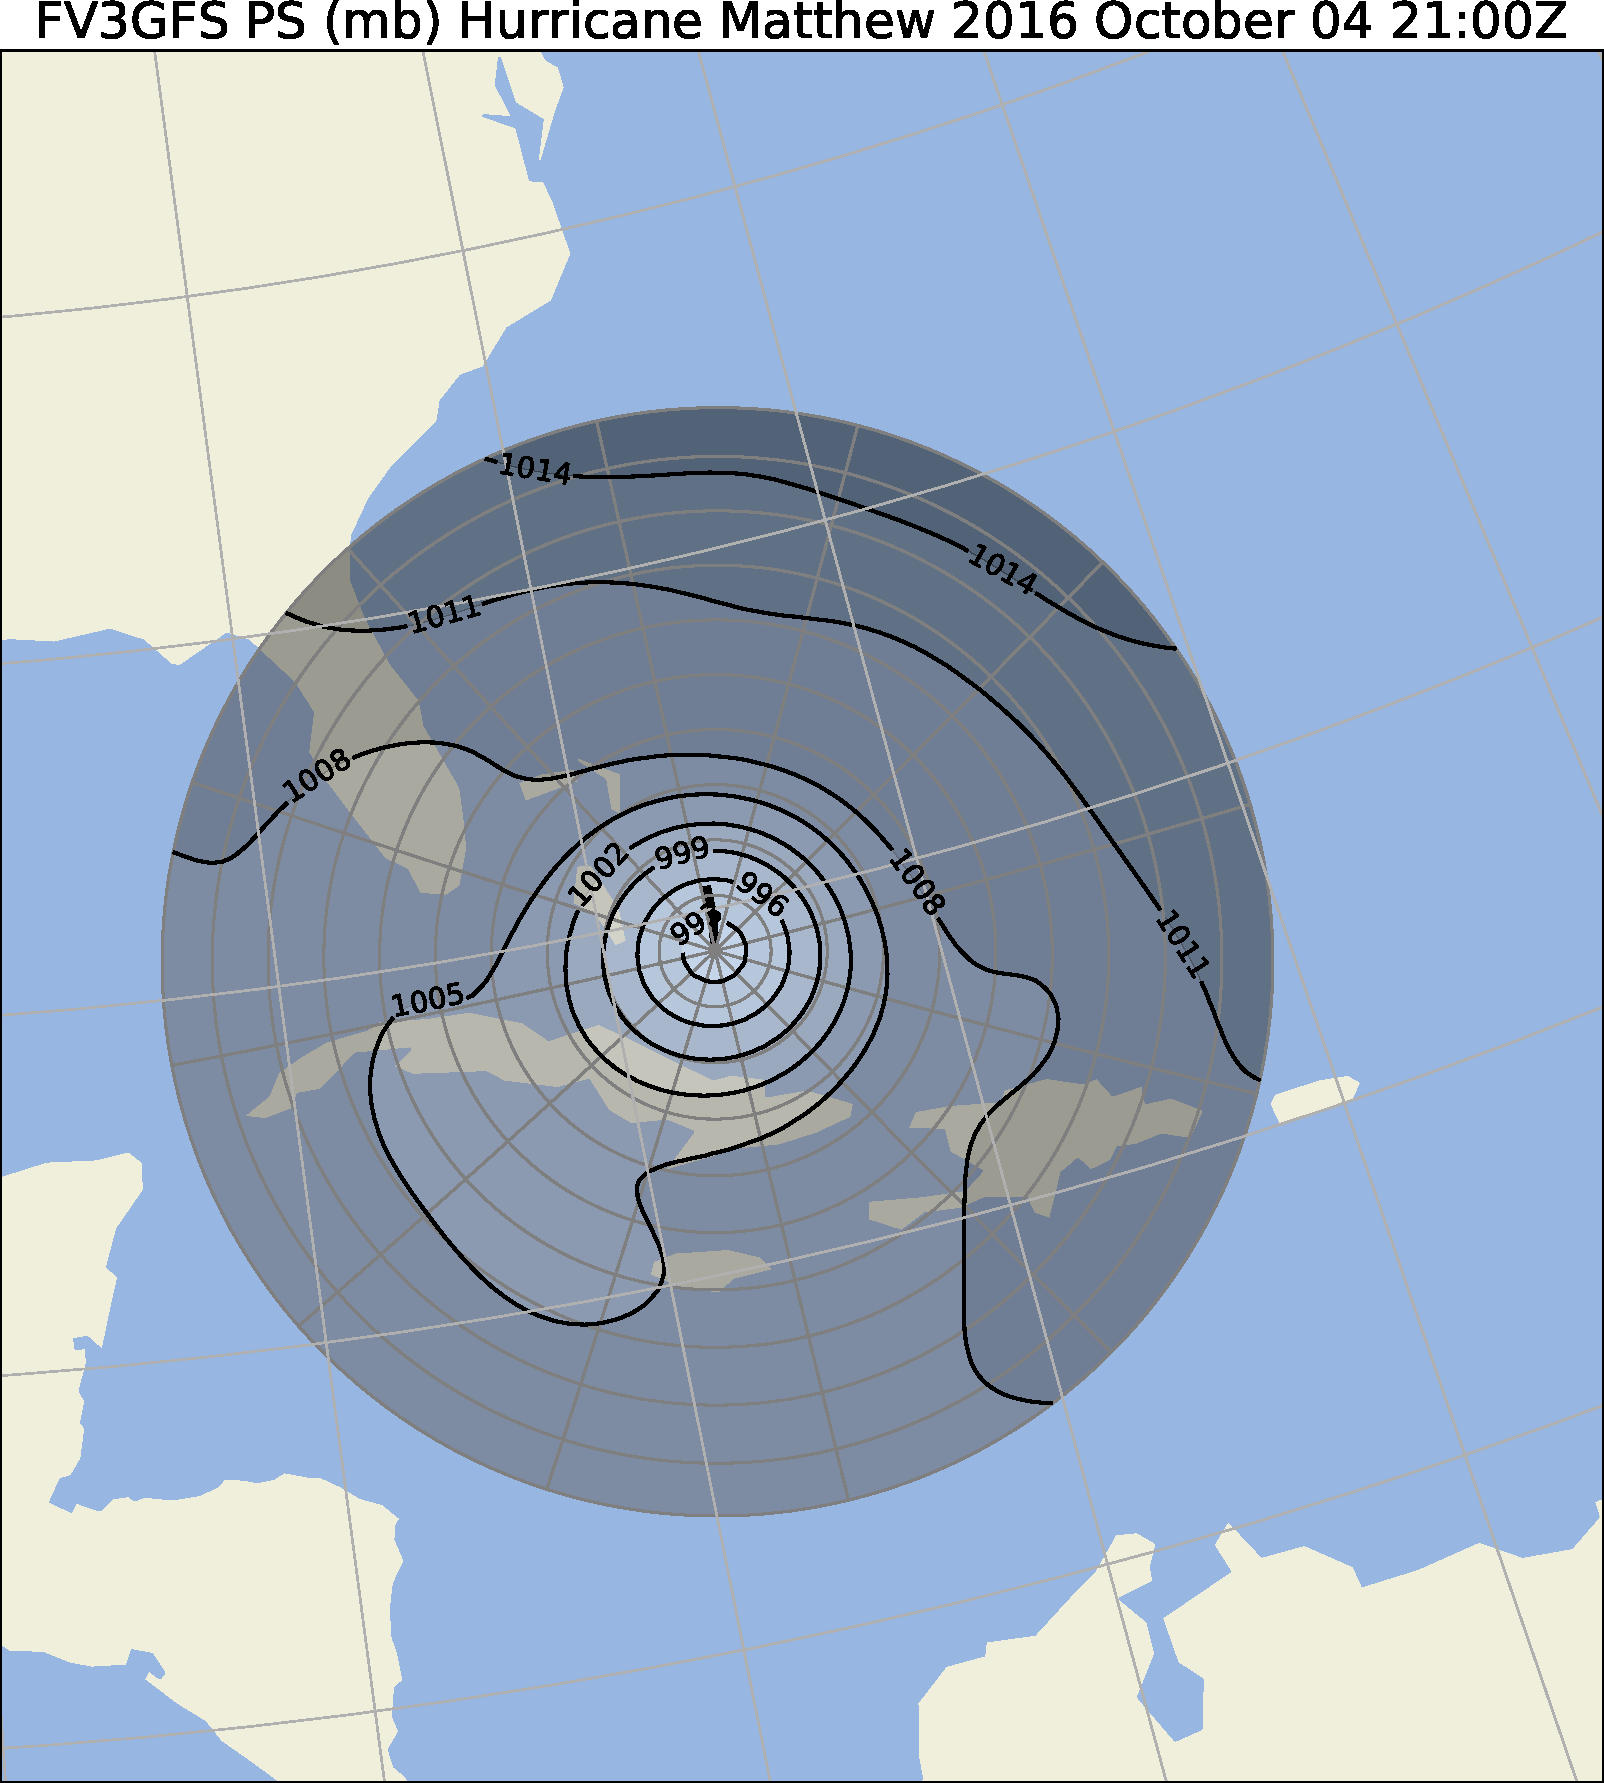
\includegraphics[width=1.0\linewidth]{../plots/PRMSL_2016100421.pdf}
\end{figure}
\begin{figure}
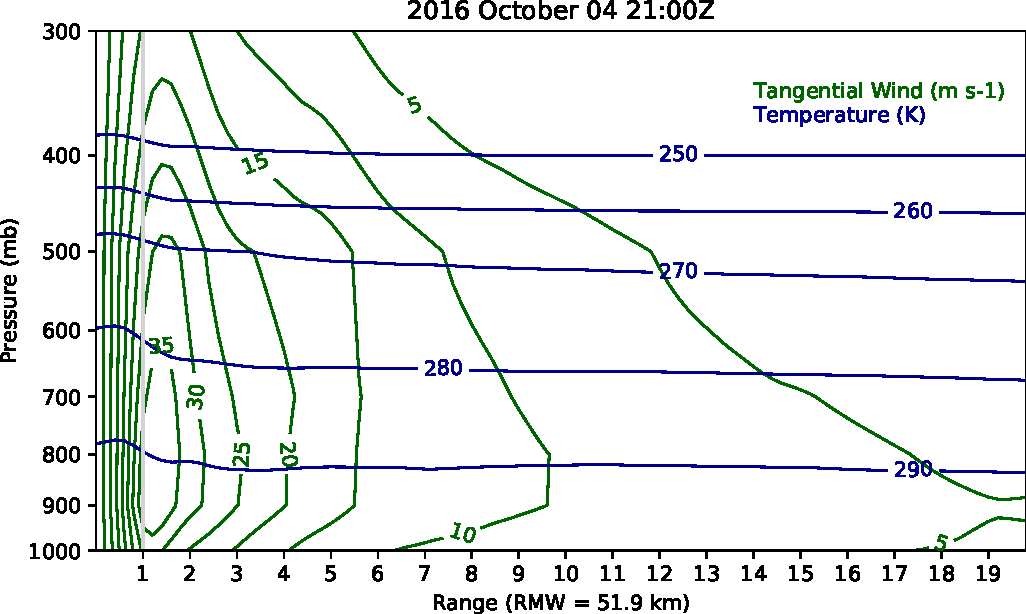
\includegraphics[width=1.0\linewidth]{../plots/cross_section_2016100421.pdf}
\end{figure}

\end{block}

%----------------------------------------------------------------------------------------

\end{column} % End of column 2.1

\begin{column}{\onecolwid} % The second column within column 2 (column 2.2)

%----------------------------------------------------------------------------------------
% RMW Analysis
%----------------------------------------------------------------------------------------

\begin{block}{RMW Analysis}

\begin{itemize}
\item Process a collection of TC RMW of NetCDF output fields,
aggregate statistics on a common range (RMW) - azimuth grid
\item Filter collection by ATCF track information, e.g. category, size,
position, valid time range, lead time, min pressure, max wind, \ldots
\end{itemize}
\vspace{1in}
\begin{figure}
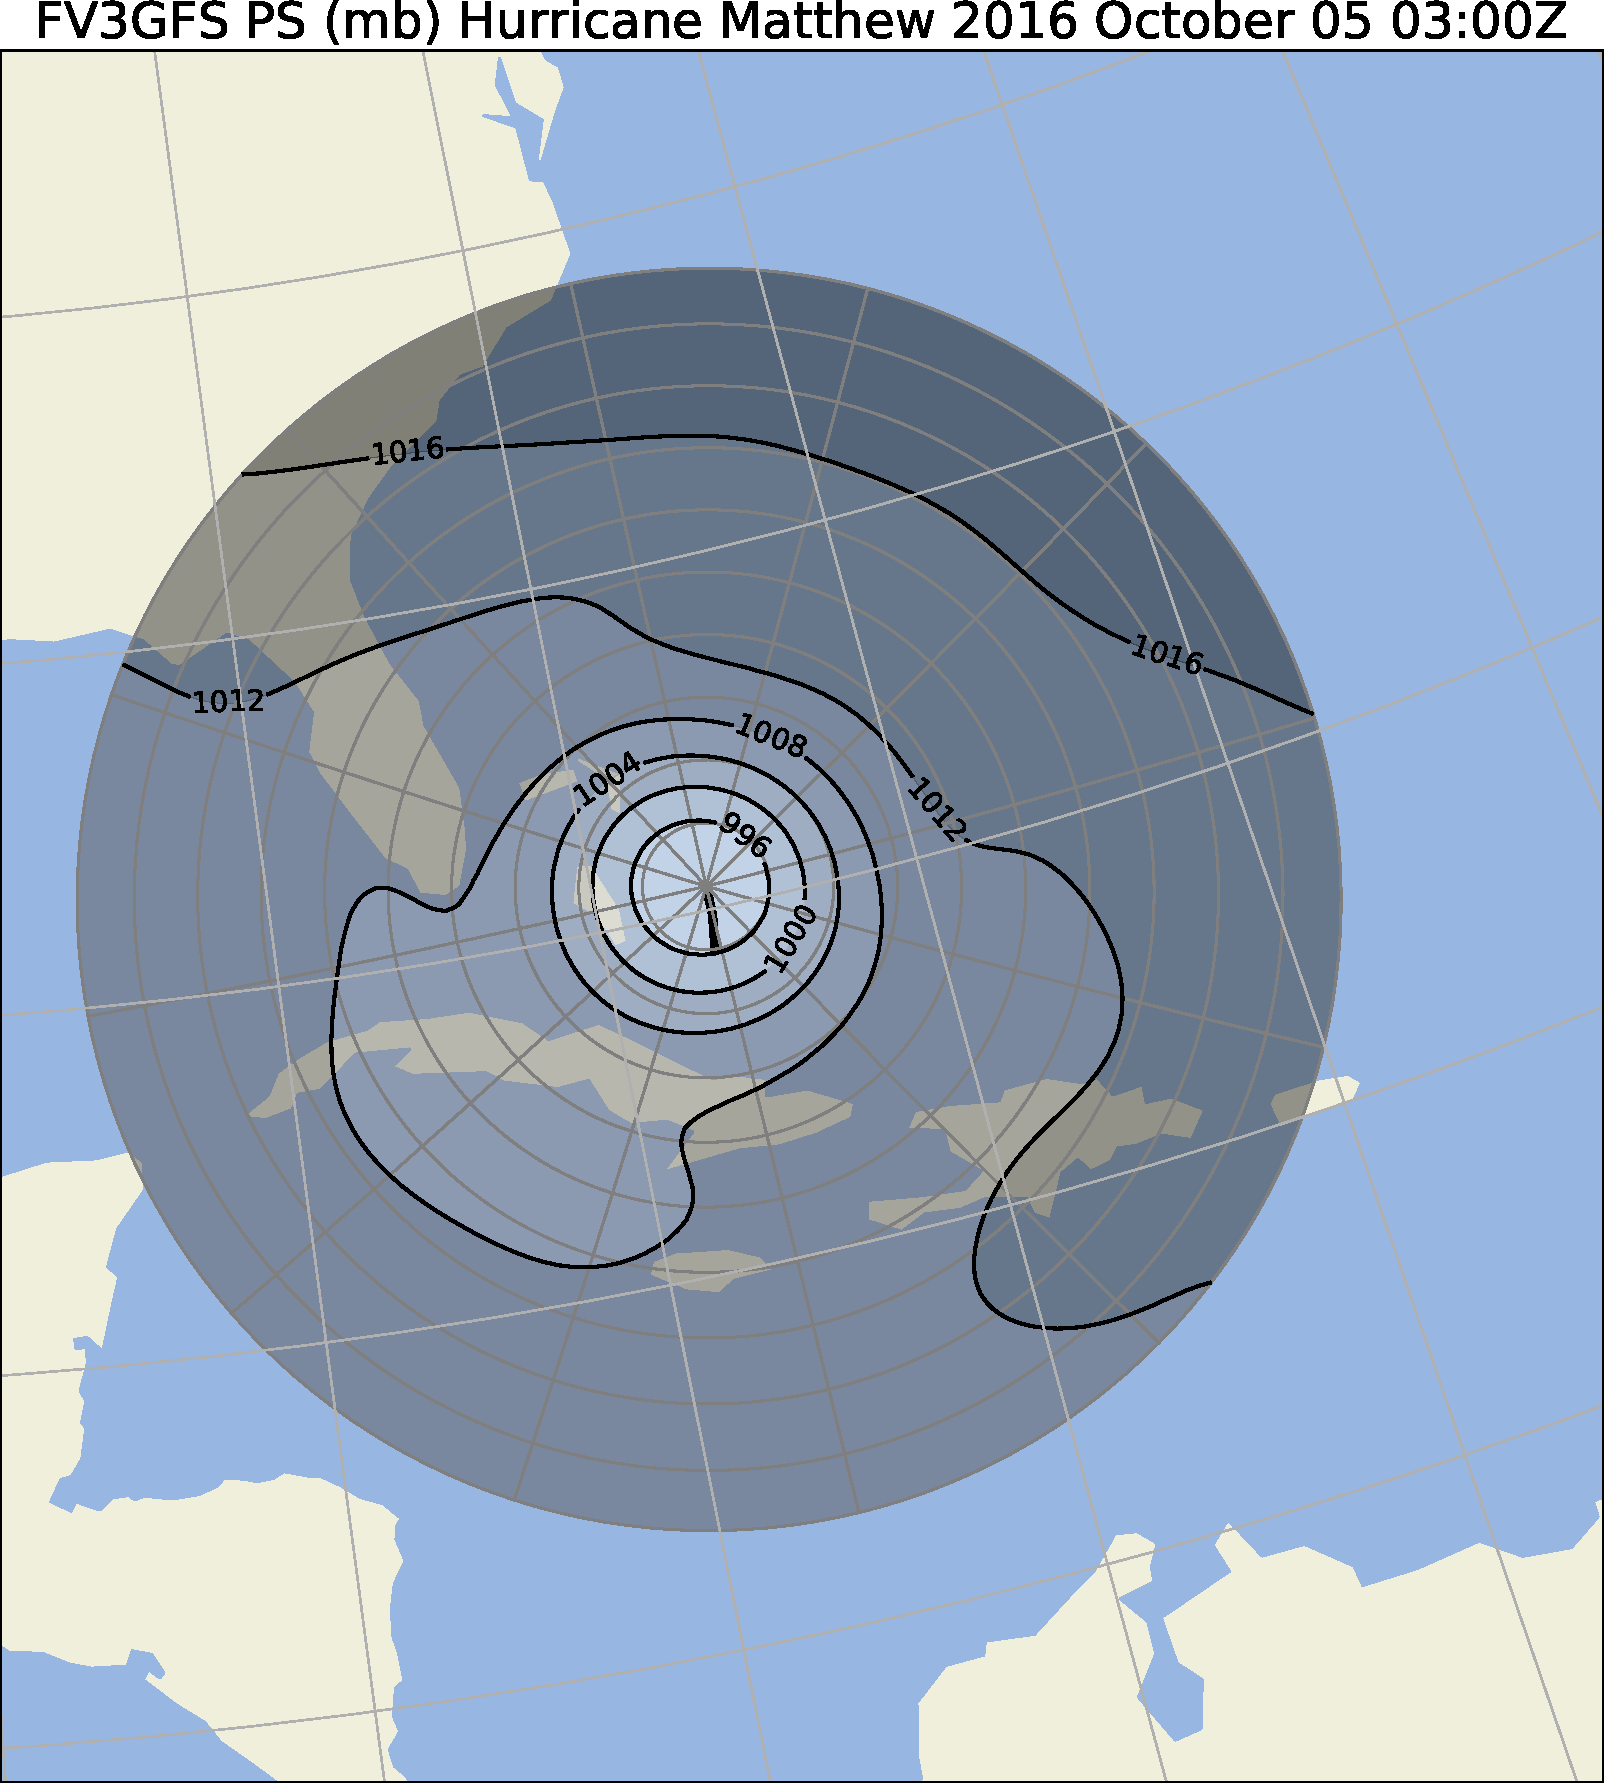
\includegraphics[width=1.0\linewidth]{../plots/PRMSL_2016100503.pdf}
\end{figure}
\begin{figure}
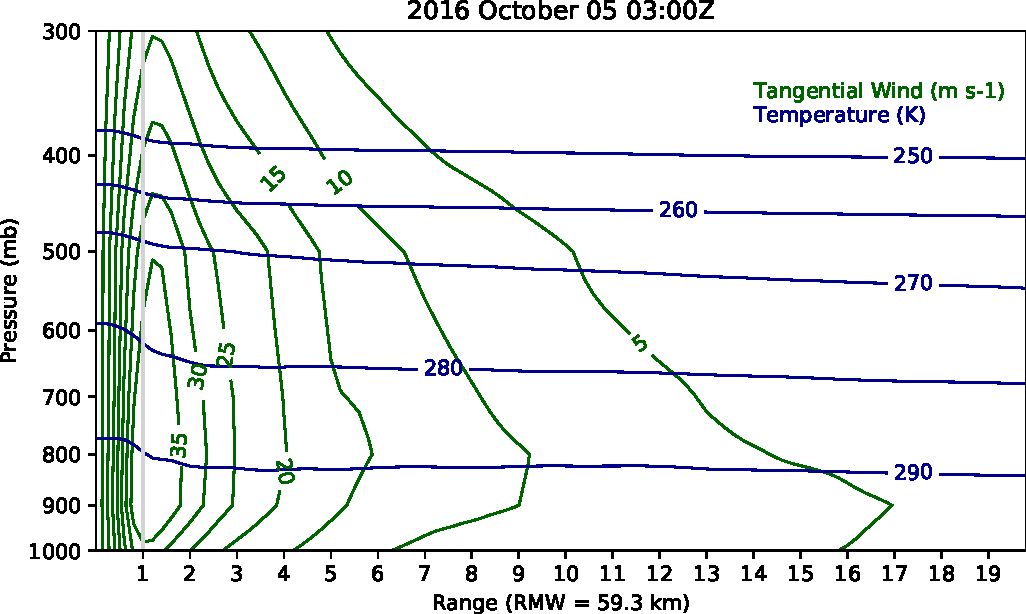
\includegraphics[width=1.0\linewidth]{../plots/cross_section_2016100503.pdf}
\end{figure}

\end{block}

%----------------------------------------------------------------------------------------

\end{column} % End of column 2.2

\end{columns} % End of the split of column 2

\end{column} % End of the second column

\begin{column}{\sepwid}\end{column} % Empty spacer column

\begin{column}{\onecolwid} % The third column

\begin{block}

\begin{lstlisting}[language=Python]
data = {
    field = [
        {
          name = "PRMSL";
          level = ["L0"];
        },
        {
          name = "TMP";
          level = ["P1000", "P950", "P900", ...];
        },
        {
          name = "UGRD";
          level = ["P1000", "P950", "P900", ...];
        },
        ...
    ];
\end{lstlisting}

\end{block}

%----------------------------------------------------------------------------------------
% REFERENCES
%----------------------------------------------------------------------------------------

\begin{block}

\nocite{*} % Insert publications even if they are not cited in the poster
\small{\bibliographystyle{unsrt}
\bibliography{sample}\vspace{0.75in}}

\end{block}

%----------------------------------------------------------------------------------------
%	CONTACT INFORMATION
%----------------------------------------------------------------------------------------

% \setbeamercolor{block alerted title}{fg=black,bg=norange} % Change the alert block title colors
% \setbeamercolor{block alerted body}{fg=black,bg=white} % Change the alert block body colors

\begin{alertblock}{Contact Information}

\begin{itemize}
\item Web: \href{https://github.com/NCAR/MET}{https://github.com/NCAR/MET}
\item Email: \href{mailto:fillmore@ucar.edu}{fillmore@ucar.edu}
\end{itemize}

\end{alertblock}

\begin{center}
% \begin{tabular}{ccc}

\includegraphics[width=0.8\linewidth]{../logos/NCAR-contemp-logo-blue.png}
% \end{tabular}
\end{center}

%----------------------------------------------------------------------------------------

\end{column} % End of the third column

\end{columns} % End of all the columns in the poster

\end{frame} % End of the enclosing frame

\end{document}
